%%%%%%%%%%%%%%%%%%%%%%%%%%%%%%%%%%%%%%%%%
% Beamer Presentation
% LaTeX Template
% Version 1.0 (10/11/12)
%
% This template has been downloaded from:
% http://www.LaTeXTemplates.com
%
% License:
% CC BY-NC-SA 3.0 (http://creativecommons.org/licenses/by-nc-sa/3.0/)
%
%%%%%%%%%%%%%%%%%%%%%%%%%%%%%%%%%%%%%%%%%

%----------------------------------------------------------------------------------------
%	PACKAGES AND THEMES
%----------------------------------------------------------------------------------------

\documentclass{beamer}

\usepackage{tikz}
\usetikzlibrary{cd}

\mode<presentation> {

% The Beamer class comes with a number of default slide themes
% which change the colors and layouts of slides. Below this is a list
% of all the themes, uncomment each in turn to see what they look like.

%\usetheme{default}
%\usetheme{AnnArbor}
%\usetheme{Antibes}
%\usetheme{Bergen}
%\usetheme{Berkeley}
%\usetheme{Berlin}
%\usetheme{Boadilla}
%\usetheme{CambridgeUS}
%\usetheme{Copenhagen}
%\usetheme{Darmstadt}
%\usetheme{Dresden}
%\usetheme{Frankfurt}
%\usetheme{Goettingen}
%\usetheme{Hannover}
%\usetheme{Ilmenau}
%\usetheme{JuanLesPins}
%\usetheme{Luebeck}
%\usetheme{Madrid}
%\usetheme{Malmoe}
%\usetheme{Marburg}
\usetheme{Montpellier}
%\usetheme{PaloAlto}
%\usetheme{Pittsburgh}
%\usetheme{Rochester}
%\usetheme{Singapore}
%\usetheme{Szeged}
%\usetheme{Warsaw}

% As well as themes, the Beamer class has a number of color themes
% for any slide theme. Uncomment each of these in turn to see how it
% changes the colors of your current slide theme.

%\usecolortheme{albatross}
%\usecolortheme{beaver}
%\usecolortheme{beetle}
%\usecolortheme{crane}
\usecolortheme{dolphin}
%\usecolortheme{dove}
%\usecolortheme{fly}
%\usecolortheme{lily}
%\usecolortheme{orchid}
%\usecolortheme{rose}
%\usecolortheme{seagull}
%\usecolortheme{seahorse}
%\usecolortheme{whale}
%\usecolortheme{wolverine}

%\setbeamertemplate{footline} % To remove the footer line in all slides uncomment this line
\setbeamertemplate{footline}[page number] % To replace the footer line in all slides with a simple slide count uncomment this line

\setbeamertemplate{navigation symbols}{} % To remove the navigation symbols from the bottom of all slides uncomment this line
}

\usepackage{graphicx} % Allows including images
\usepackage{subfig} % Allows including images
\usepackage{booktabs} % Allows the use of \toprule, \midrule and \bottomrule in tables
\usepackage[backend=biber, sorting=none]{biblatex}
\addbibresource{sources.bib}

\AtBeginSection[]
{
    \begin{frame}
        \frametitle{Table of Contents}
        \tableofcontents[currentsection]
    \end{frame}
}
%----------------------------------------------------------------------------------------
%	TITLE PAGE
%----------------------------------------------------------------------------------------

\title[]{TLA+ and a Concurrent Hashmap Specification} % The short title appears at the bottom of every slide, the full title is only on the title page

\author{Åsmund Aqissiaq Arild Kløvstad} % Your name
\institute[UiB] % Your institution as it will appear on the bottom of every slide, may be shorthand to save space
{
Universitetet i Bergen \\ % Your institution for the title page
}
\date{\today} % Date, can be changed to a custom date

\begin{document}

\begin{frame}
\titlepage % Print the title page as the first slide
\end{frame}

% \begin{frame}
% \frametitle{Overview} % Table of contents slide, comment this block out to remove it
% \tableofcontents % Throughout your presentation, if you choose to use \section{} and \subsection{} commands, these will automatically be printed on this slide as an overview of your presentation
% \end{frame}

%----------------------------------------------------------------------------------------
%	PRESENTATION SLIDES
%----------------------------------------------------------------------------------------

%------------------------------------------------
% \section{Some Intro Stuff} % Sections can be created in order to organize your presentation into discrete blocks, all sections and subsections are automatically printed in the table of contents as an overview of the talk
% %------------------------------------------------

%------------------------------------------------

\section{Introduction}

%------------------------------------------------

\begin{frame}
  \frametitle{Outline}
  \begin{enumerate}
  \item The project
  \item The data structure
  \item TLA+
  \item The specification
  \item Results and lessons learned
  \end{enumerate}
\end{frame}

%------------------------------------------------

\begin{frame}
  \frametitle{The Project}
  \begin{itemize}
  \item 10 pt optional Bachelor Thesis at UiT
  \item Spring semester 2020
  \item Supervised by Håvard D. Johansen
  \item Specifying and modelchecking a hash table in TLA+
  \end{itemize}
\end{frame}
%------------------------------------------------

\begin{frame}
  \frametitle{Problem Statement}
  \begin{itemize}
  \item Formal methods
  \item Concurrent and distributed systems
  \item A novel hashmap~\cite{Shalev2006}
  \end{itemize}
  \vfill{}
  \begin{quotation}
    Shalev et. al.'s Hash Table can be formally verified for concurrent settings
  \end{quotation}
\end{frame}

\section{The Hashmap}

%------------------------------------------------

\begin{frame}
  \frametitle{The Idea}
  \begin{itemize}
  \item Resizing is hard in concurrent settings
  \item Solution: move the buckets instead
  \item Split-ordering (sort by reverse binary representation)
  \item Dummy nodes
  \end{itemize}

  \begin{figure}
    \centering
    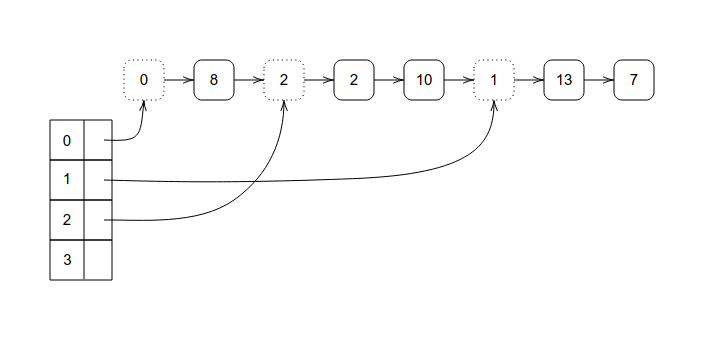
\includegraphics[width=\textwidth]{figures/split-ordered-list-diagram}
    \caption{Split-ordered list}
    \label{fig:SOlist}
  \end{figure}
\end{frame}

%------------------------------------------------
\begin{frame}
  \frametitle{Insertion with Splitting}
  \begin{figure}
      \subfloat[Initial state]{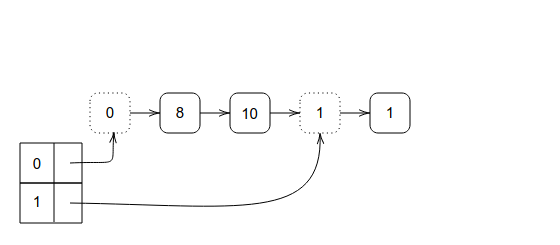
\includegraphics[height=1in]{figures/expand-0.png}}
      \subfloat[Table is expanded]{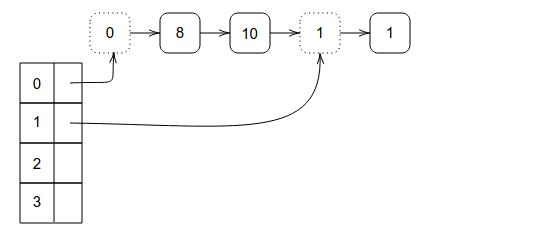
\includegraphics[height=1in]{figures/expand-1.png}}
      \newline
      \subfloat[Dummy node for new bucket inserted]{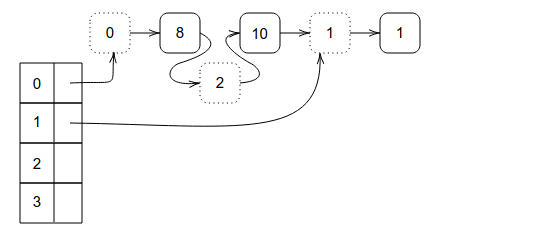
\includegraphics[height=1in]{figures/expand-2.png}}
      \subfloat[Table entry points to bucket node]{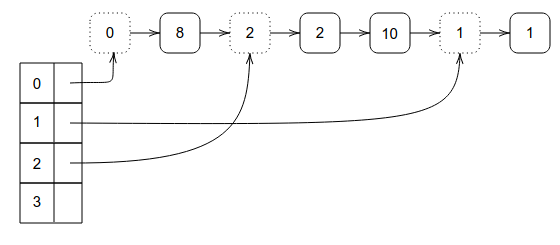
\includegraphics[height=1in]{figures/expand-3.png}}
  \caption{Expansion and bucket splitting}    
  \label{fig:insert-expand}
  \end{figure}
\end{frame}

%------------------------------------------------
\section{TLA+}

%------------------------------------------------

\begin{frame}
  \frametitle{The Basics}
  \begin{itemize}
  \item \textbf{T}emporal \textbf{L}ogic of \textbf{A}ctions
  \item Modalities: always ($\square$) and eventually ($\diamond$)
  \item \textbf{actions} are logical predicates on \textbf{variables}
  \item The basic specification ``Init and always Next'':
    \[ Spec \triangleq Init \land \square [Next]_{\langle iter, revIter
        \rangle} \]
  \item Implementation is implication. $A$ implements $B$ exactly when
    $A \implies B$
  \end{itemize}
\end{frame}

%------------------------------------------------

\begin{frame}
  \frametitle{Syntax Quirks}
  \begin{itemize}
  \item Primed variables
    \[ Next \triangleq iter' = iter + 1 \land \text{UNCHANGED } revIter \]
  \item Functions
    \[ list \triangleq [0..42 \mapsto String] \]
  \item EXCEPT
    \[ list' = [list \text{ EXCEPT } ![4] = "hei"] \]
  \end{itemize}
\end{frame}

%------------------------------------------------

\section{The Formalization}

%------------------------------------------------
\begin{frame}
  \frametitle{Overview}
  Four specifications:
  \begin{enumerate}
  \item Generic hash table\label{item:generic}
  \item Non-concurrent split-order implementing \autoref{item:generic}.
  \item Concurrent split-order
  \item (Concurrent with operation ID's)
  \end{enumerate}
\end{frame}

%------------------------------------------------
\begin{frame}
  \frametitle{Generic Hash Table}
  \begin{figure}
    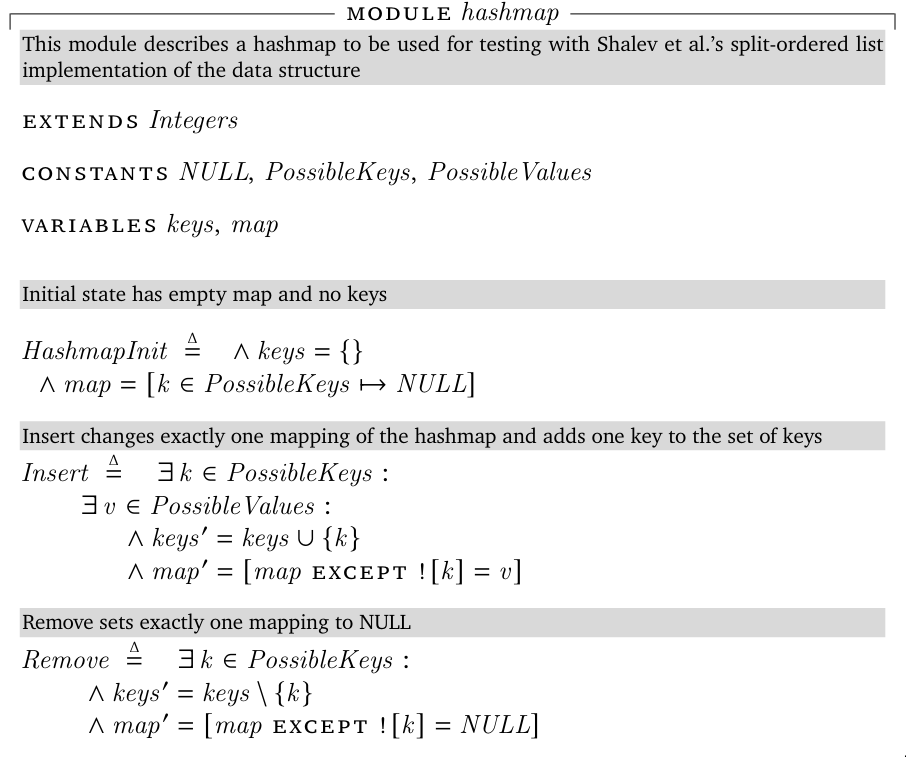
\includegraphics[height=.7\paperheight]{figures/generic}
    \caption{Generic hash table specification}
    \label{fig:generic}
  \end{figure}
\end{frame}

%------------------------------------------------

\begin{frame}
  \frametitle{Non-concurrent}
  \begin{figure}
    \centering
    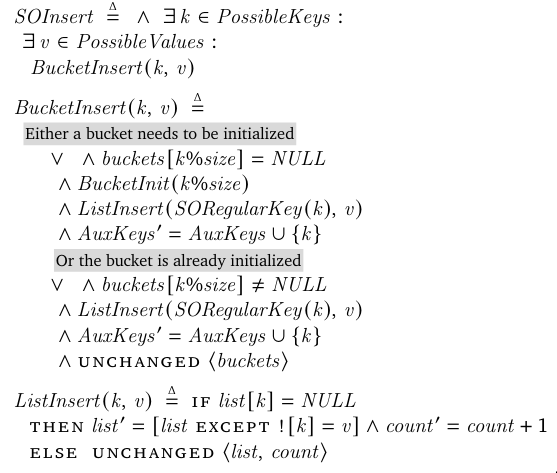
\includegraphics[height=.7\paperheight]{figures/insert-spec}
    \caption{The insert operation}
    \label{fig:insert}
  \end{figure}
\end{frame}

%------------------------------------------------

\begin{frame}[allowframebreaks]
  \frametitle{Concurrent Operations}
  \begin{figure}
    \captionsetup[subfigure]{labelformat=empty}
      \subfloat[Next step]{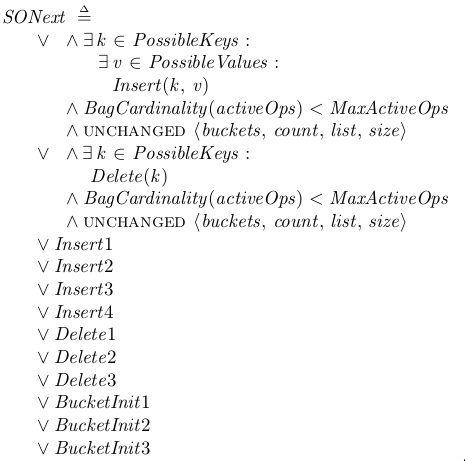
\includegraphics[height=2in]{figures/concurrent-next.png}}
      \newline
      \subfloat[]{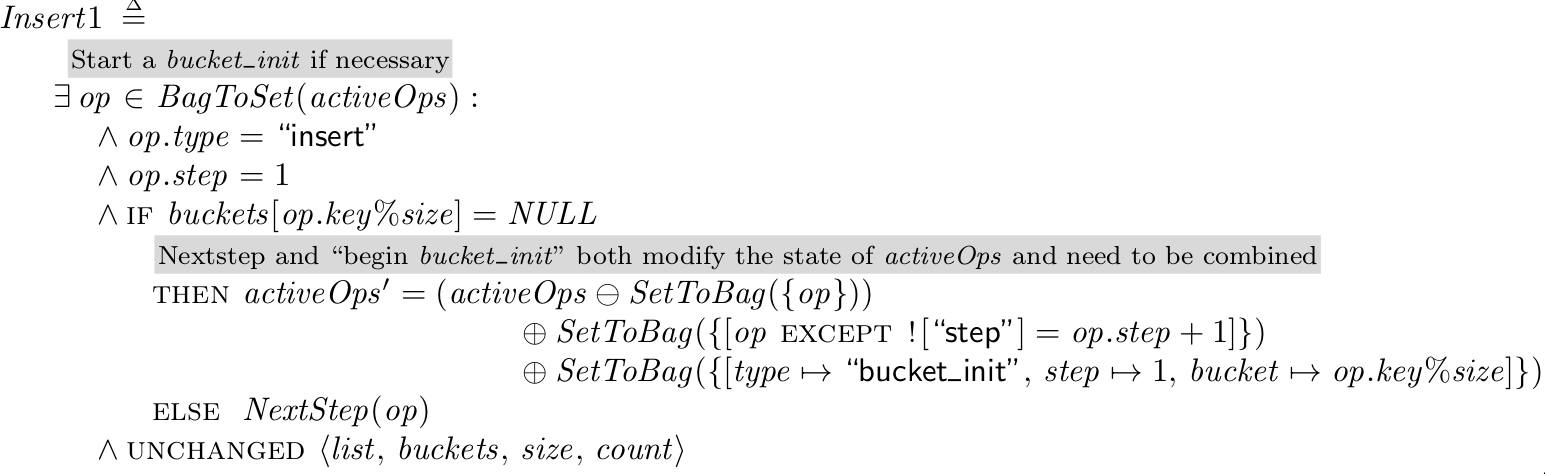
\includegraphics[height=1in]{figures/insert1}}
      \newline
      \subfloat[]{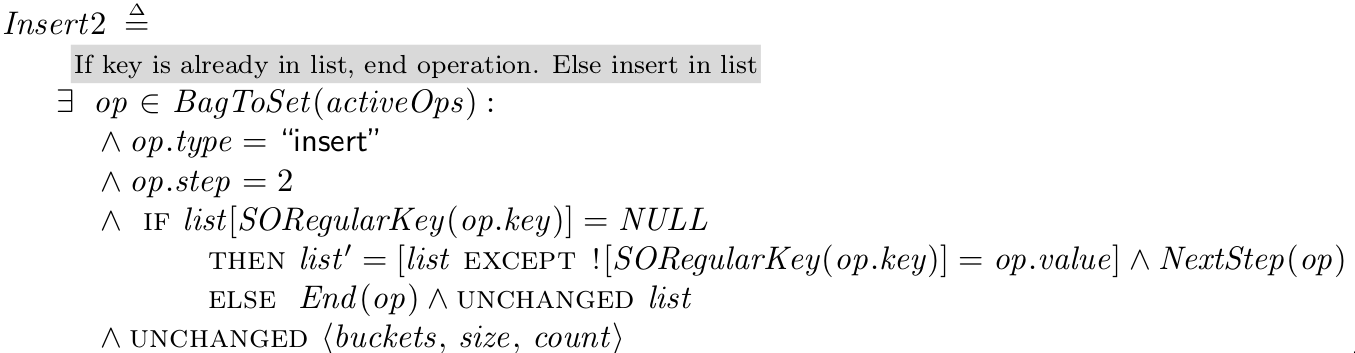
\includegraphics[height=1in]{figures/insert2.png}}
      \newline
      \subfloat[]{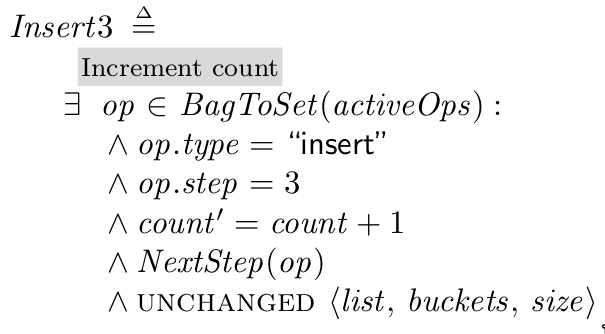
\includegraphics[height=1in]{figures/insert3.png}}
      \newline
      \subfloat[]{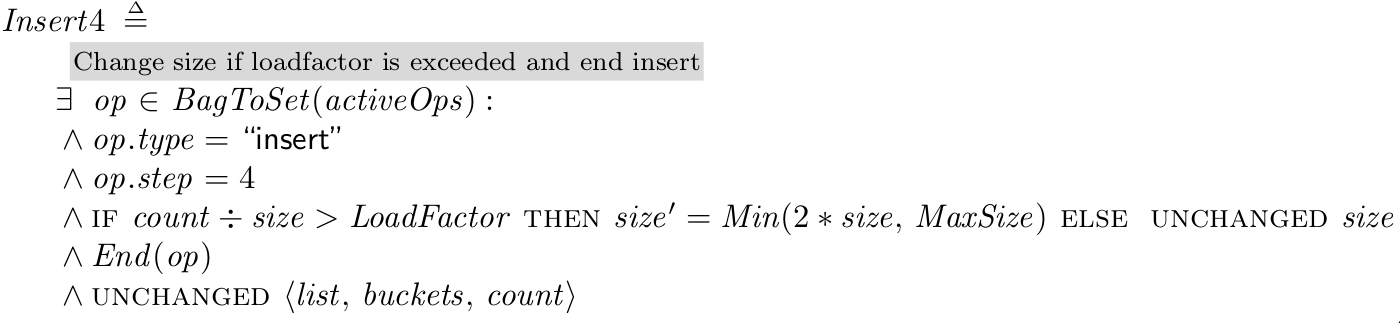
\includegraphics[height=1in]{figures/insert4.png}}
  \label{fig:insert-concurrent}
  \end{figure}
\end{frame}
%------------------------------------------------

\begin{frame}
  \frametitle{Testing the Non-concurrent Spec}
  \[ SOSpec \triangleq SOInit \land \square [SONext]_{\langle {keys, AuxKeys,
        list, buckets, size, count, map} \rangle}
    \\
    \text{INSTANCE } hashmap
    \\
    \text{THEOREM } SOSpec \implies HashmapSpec \]

\end{frame}
%------------------------------------------------
\begin{frame}[allowframebreaks]
  \frametitle{Testing the Specifications}
  Claimed invariants:
  \begin{enumerate}
  \item If a bucket is initialized, then it points to a dummy node in the list
    \begin{figure}
    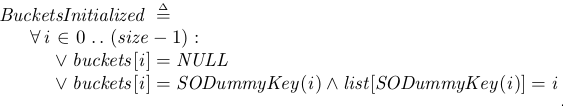
\includegraphics[width=.8\textwidth]{figures/bucketsinitialized}
    \end{figure}
  \item If $k$ is not in the map, then \texttt{delete(k)} fails. Otherwise $k$ is
    removed from the map
    \begin{figure}[h]
    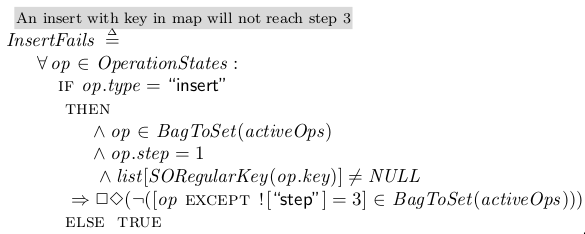
\includegraphics[width=.8\textwidth]{figures/insertfails}
    \end{figure}
  \item If $k$ is in the map, then \texttt{insert(k)} fails. Otherwise $k$ is
    added to the map
  \end{enumerate}
\end{frame}

\section{Results}

%------------------------------------------------
\begin{frame}
  \frametitle{Non-concurrent}
\begin{table}[h]
    \centering
    \begin{tabular}{ |c|c||c|c|c| }
        \hline
        Keys & Values & Diameter & Distinct & Time \\
        &        &          & States   & (hh:mm:ss)\\
        \hline
        2 & 4  & 10 & 2,523      & 00:00:01\\
        2 & 8  & 10 & 23,763     & 00:00:08\\
        2 & 16 & 10 & 279,075    & 00:01:02\\
        4 & 2  & 17 & 39,827     & 00:00:09\\
        4 & 4  & 17 & 1,790,067  & 00:03:44\\
        4 & 8  & 17 & 147,266,723& 07:14:45\\
        \hline
    \end{tabular}
    \caption{Model checking results for SplitOrder}
    \label{tab:SplitOrder}
\end{table}
\end{frame}

\begin{frame}
  \frametitle{Concurrent}
\begin{table}[h]
  \centering
    \resizebox{!}{1.5in}{%        
    \begin{tabular}{ |L|c|c|c||c|c|c| }
        \hline
        Invariant & Keys & Values & Conc. & Diameter & Distinct & Time\\
        &      &        & Ops        &          & States   & (mm:ss)\\
        \hline
        \textit{InsertSucceeds} & 2 & 2 & 2 & 38 & 10,083    & 00:02\\
        & 2 & 4 & 2 & 38 & 66,901    & 00:13\\
        & 2 & 4 & 3 & 45 & 1,351,453 & 01:50\\
        & 4 & 2 & 2 & 62 & 1,627,390 & 02:15\\
        \hline
        \textit{DeleteSucceeds} & 2 & 2 & 2 & 38 & 10,083    & 00:01\\
        & 2 & 4 & 2 & 38 & 66,901    & 00:07\\
        & 2 & 4 & 3 & 45 & 1,351,453 & 00:31\\
        & 4 & 2 & 2 & 62 & 1,627,390 & 00:45\\
        \hline
        \textit{BucketsInitialized} & 2 & 2 & 2 & 38 & 10,083    & 00:02\\
        & 2 & 4 & 2 & 38 & 66,901    & 00:16\\
        & 2 & 4 & 8 & 38 & 624,645   & 00:16\\
        & 2 & 4 & 16& 38 & 7,371,157 & 01:55\\
        & 4 & 2 & 2 & 62 & 1,627,390 & 00:22\\
        & 4 & 3 & 2 & 62 & 8,368,282 & 01:39\\
        & 4 & 4 & 2 & 62 & 29,973,646& 06:10\\
        & 4 & 5 & 2 & 62 & 85,419,916& 18:41\\
        & 4 & 2 & 3 & 75 & 61,353,460& 13:59\\
        \hline
    \end{tabular}}
  \end{table}
\end{frame}

\begin{frame}
  \frametitle{Failures}
  
\begin{table}
    \centering
    \resizebox{\textwidth}{!}{%
        \begin{tabular}{ |L|L|c|c|c||c|c|c|p{1cm}| }
        \hline
        Invariant & Keys & Values & Conc. & Diameter & Distinct & Time & Error\\
                  &      &        & Ops   &          & States   & (hh:mm:ss)&\\
        \hline
        Non-Concurrent   &4      & 16     &       &17 & 84,587,043 & 02:54:11 & 3\\
        \hline
        \textit{InsertSucceeds}& 4 & 3 & 2 & 27 & 1,426,888 & 00:33:30 & 2\\
        \hline
        \textit{DeleteSucceds}& 4 & 3 & 2 & 39 & 6,067,795 & 00:30:30 & 1\\
        \hline
        \textit{BucketsInitialized}& 4 & 2 & 4 & 57 &120,175,837& 00:26:49 &4\\
        \hline
    \end{tabular}}
    \caption{Failed model checks}
    \label{tab:failed-checks}
\end{table}
\begin{table}
    \centering
    \begin{tabular}{ |L|L| }
        \hline
        Code & Error\\
        \hline
        1 & GC Overhead limit exceeded\\
        2 & Out of heap space\\
        3 & No space left on device\\
        4 & Unknown\\
        \hline
    \end{tabular}
    \caption{Error Codes}
    \label{tab:errors}
\end{table}
\end{frame}

\section{Lessons Learned and Conclusion}
\begin{frame}
  \frametitle{Designing Specifications}
  \begin{enumerate}
  \item Decide on purpose early and precisely
  \item Choose step size early and deliberately
  \item Test assumed invariants and try to break them
  \end{enumerate}
  
\end{frame}
\begin{frame}
  \frametitle{The Use of Model Checking}
  \begin{itemize}
  \item Poor scaling
  \item Computationally expensive
  \item Useful
    \begin{enumerate}
    \item as a way  to produce minimal examples of errors, and
    \item as a development tool for algorithms/protocols
    \end{enumerate}
  \item Increased confidence in algorithms, though arguably no more than a
    tested implementation
  \end{itemize}
\end{frame}

%------------------------------------------------
\begin{frame}
  \frametitle{References}
  Tables and figures from my bachelor thesis~\cite{Klovstad2020}
  \printbibliography{}
\end{frame}

\end{document} 